% \begin{figure}[h]
% \centering
% %
% \subfloat[
%     \textbf{CIFAR-100 (50+50).}
%     \label{fig:data_use_cifar100}
% ]{
% \centering
% \begin{minipage}{0.48\linewidth}{
% \begin{center}
%     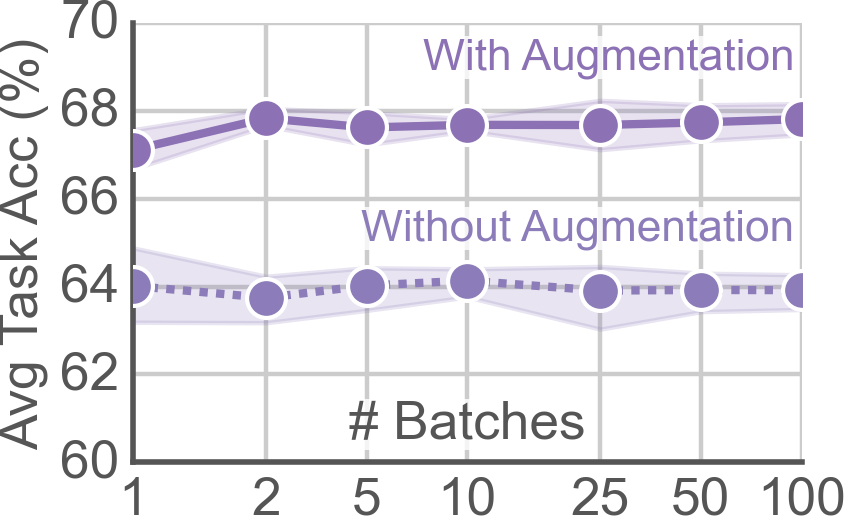
\includegraphics[width=\linewidth]{figures/imgs/cifar100_data.png}
% \end{center}
% }\end{minipage}
% }
% \subfloat[
%     \textbf{ImageNet-1k (200+200).}
%     \label{fig:data_use_imagenet}
% ]{
% \centering
% \begin{minipage}{0.48\linewidth}{
% \begin{center}
%     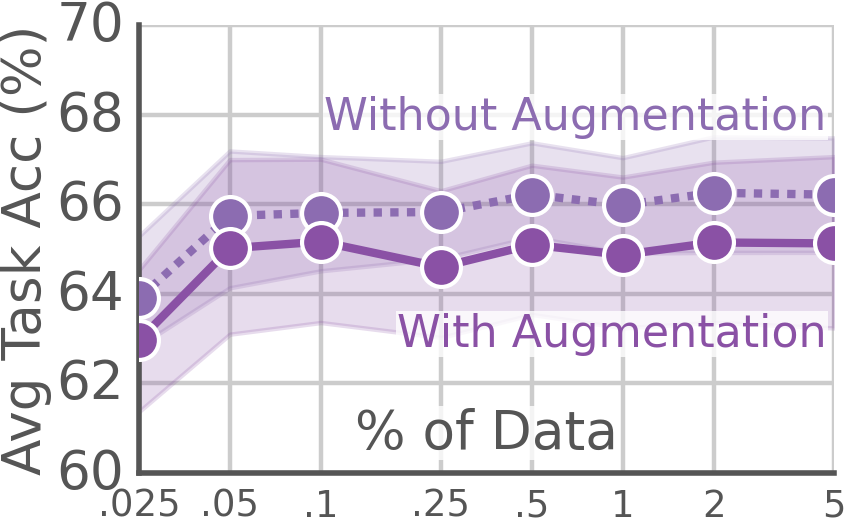
\includegraphics[width=\linewidth]{figures/imgs/imnet200_data.png}
% \end{center}
% }\end{minipage}
% }

% \caption{{\bf Data Usage.} How much data do we need to use to compute activations? Here we ablate the amount of data used for our CIFAR-100 (50+50) ResNet-20 ($8\times$ width) and ImageNet (200+200) Resnet-50 (\sfrac{22}{50} layers) experiments. The batch size used is 500 for CIFAR and 16 for ImageNet. In both cases, we only need a few hundred images to obtain the best results. On the other hand, data augmentation is necessary for CIFAR but hurts for ImageNet. Our default for all experiments uses data augmentation and the full set for CIFAR (100 batches) and 1\% of the data for ImageNet. }
% \label{fig:data_usage}
% \end{figure}



% \begin{wrapfigure}{l}{0.52\linewidth}
% % \vspace{-260pt}
% \begin{minipage}[l]{\linewidth}{
% \subfloat[
%     \textbf{CIFAR-100 (50+50).}
%     \label{fig:data_use_cifar100}
% ]{
% \centering
% \begin{minipage}{0.48\linewidth}{
% \begin{center}
%     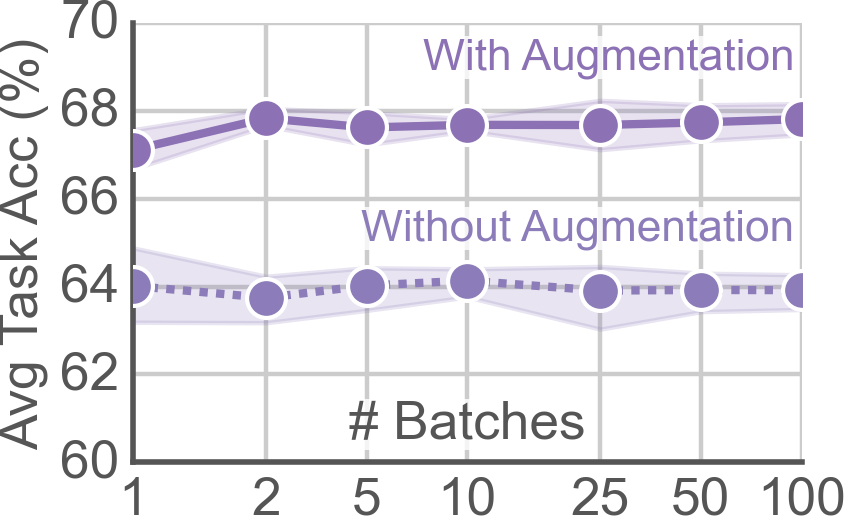
\includegraphics[width=\linewidth]{figures/imgs/cifar100_data.png}
% \end{center}
% }\end{minipage}
% }
% \subfloat[
%     \textbf{ImageNet-1k (200+200).}
%     \label{fig:data_use_imagenet}
% ]{
% \centering
% \begin{minipage}{0.48\linewidth}{
% \begin{center}
%     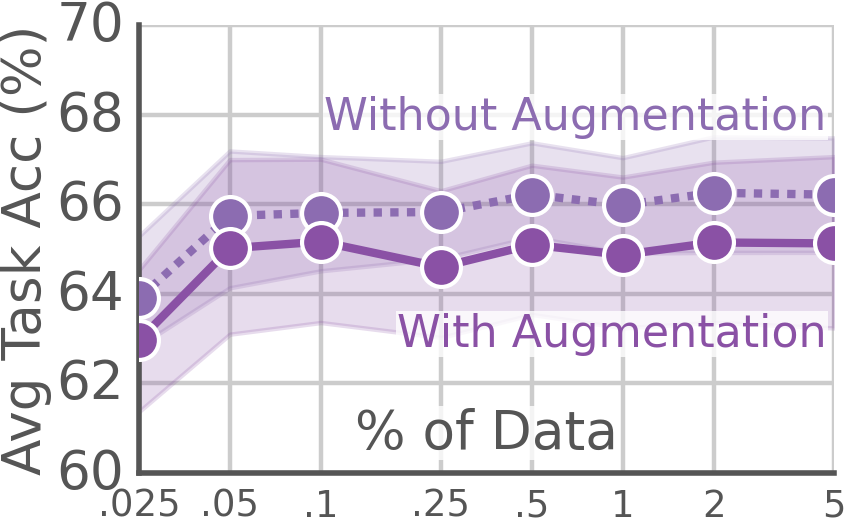
\includegraphics[width=\linewidth]{figures/imgs/imnet200_data.png}
% \end{center}
% }\end{minipage}
% }
%         \caption{
%         {\bf Data Usage.} How much data do we need to use to compute activations? Here we ablate the amount of data used for our CIFAR-100 (50+50) ResNet-20 ($8\times$ width) and ImageNet (200+200) Resnet-50 (\sfrac{22}{50} layers) experiments. The batch size used is 500 for CIFAR and 16 for ImageNet. In both cases, we only need a few hundred images to obtain the best results. On the other hand, data augmentation is necessary for CIFAR but hurts for ImageNet. Our default for all experiments uses data augmentation and the full set for CIFAR (100 batches) and 1\% of the data for ImageNet. 
%         }
% \label{fig:data_usage}
% }\end{minipage}
% \end{wrapfigure}